\chapter{Methods}
\label{chapter:methods}
This chapter discusses the design of the study. First, research questions are introduced.
Second, research hypothesis is made based on the reviewed practices \& related research findings introduced in the chapter \ref{chapter:background}
and features of studied testing frameworks explained in chapter \ref{chapter:environment}.
Third, the empirical study and its methodology are explained in detail.

\section{Research questions}
This thesis studies low-level testing done with xUnit family testing framework	\textit{JUnit}  and how it changes after putting
an implementation level BDD-testing framework into operation. The scope in research is testing Java-code. The following
research questions are aimed to highlight the change in low-level testing after the testing framework change:
\begin{addmargin}[2em]{0em}
\vspace{20px}
\begin{itemize}
\item[\textbf{RQ1:}] How does behavior-driven testing frameworks change developer practices working with automated low-level testing compared to	\textit{JUnit}  framework?
\item[\textbf{RQ2:}] How does behavior-driven testing frameworks change developer perception of working with automated low-level testing compared to \textit{JUnit}  framework?
\item[\textbf{RQ3:}] How does behavior-driven testing frameworks change written low-level test cases and test code coverage compared to \textit{JUnit}  framework?
\end{itemize}
\end{addmargin}

\section{Research hypotheses}
    The following hypotheses are derived from the mentioned benefits of BDD literature in chapter \ref{chapter:background} and features of BDD
    testing frameworks illustrated in previous chapter. These hypotheses adhere directly to most common problems found in unit
    testing practitioner research mentioned in section \ref{section:research} in chapter \ref{chapter:background}:
    \textit{readibility} of unit tests is not optimal, \textit{maintainability} of unit tests is problematic and \textit{enjoyment}
    in practicing unit testing is low.
    \begin{addmargin}[0em]{0em}
    \vspace{10px}
    \textbf{Hypothesis 1 (H1):} Developers will write more granular test cases
    \vspace{5px}
    \newline
    As has been noted before in benefits of implementation level behavior-driven development, BDD-testing frameworks operating on this
    level aim to produce granular test cases with descriptive named test methods~\cite{chelimsky2010rspec, astels2006new, kapelonis2016java}.
    For example RSpec was originally intended to help the shifting of viewpoint from 1-1 relationship between test-code
    and only one test method per function to more granular test cases~\cite{astels2006new}.
    Compared to earlier average in the project, hypothesis should be visible in test cases through more measured test methods
    per method of component under test. In addition, the phenomena is also studied with a participant survey.
    \end{addmargin}

    \begin{addmargin}[0em]{0em}
    \vspace{10px}
    \textbf{Hypothesis 2 (H2):} Developers will find it easier to understand test cases
    \vspace{5px}
    \newline
    As stated earlier, implementation level BDD-testing frameworks should produce test cases of the component under test,
    that \textbf{describe behavior} with examples~\cite{chelimsky2010rspec}~\cite{astels2006new}~\cite{amodeo2015learning}.
    The close to natural language DSL used to create these behavior specifying tests with BDD-testing frameworks should
    have a natural tendency to "force" developers to write more descriptive tests. This is provided for example
    with xSpec family keywords \textit{describe} \& \textit{it} and with Gherkin family \textit{Given, When \& Then}-steps.
    The context, stimulus and assertions of the tests should be more visible with these mentioned structures and the test output
    should be more understandable~\cite{smart2014bdd}. Master's thesis by Laplante had also studied that BDD specifications
    was perceived by developers to produce more readable tests than the ones written with xUnit testing family tools~\cite{laplante2009behavior}.
    Hypothesis is measured with surveys, interview and with data from test code analysis.
    \end{addmargin}

    \begin{addmargin}[0em]{0em}
    \vspace{10px}
    \textbf{Hypothesis 3 (H3):} Developers will find it easier to maintain code
    \vspace{5px}
    \newline
    Implementation level BDD specifications should produce up-to-date living documentation, which can help in overall
    maintenance of the the system~\cite{smart2014bdd}. Especially the maintaining of test cases should be easier
    with repetition reducing techniques provided by these BDD-testing frameworks~\cite{chelimsky2010rspec}~\cite{kapelonis2016java}.
    xSpec family nested group examples and lifecycle hooks should allow efficient repetition removal compared to traditional xUnit family testing frameworks.
    Data Driven Testing DSL of \textit{Spock} testing framework should allow to more easily test parameter variations and remove
    the need for separate test methods, therefore making it easier to maintain the test case.
    Hypothesis is measured with surveys and interview.
    \end{addmargin}

    \begin{addmargin}[0em]{0em}
    \vspace{10px}
    \textbf{Hypothesis 4 (H4):} Developers will perceive working with low-level automated testing more enjoyable.
    \vspace{5px}
    \newline
    This hypothesis is a combination of the three earlier hypotheses. By changing the used practices and language in low-level testing,
    the overall result should appear as more enjoyable low-level testing for developers. Especially the hypotheses 2 and 3, easier understanding
    and maintaining of test cases should affect how automated low-level testing is perceived.
    Hypothesis is measured with surveys.
    \end{addmargin}

\section{Empirical study}
First in this section the type of study is determined, together with rationale and objectives of it. Second, the case selection
is explained with process for selecting teams and developers. Third, the data selection methods of this empirical study are
explained. Finally, threats to validity and limitations in this study are reviewed.

\subsection{Type of study and purpose}
    This section explains the design of the empirical \textbf{case study} collecting evidence from multiple sources with methodological triangulation.
    The data was collected from multiple projects and participants with surveys and interviews.
    Case study data collecting was enriched with observations from
    multiple projects and their test code changes. Survey data can be categorized as quantative, interview data as qualitative and observation data as quantative.
    This study follows the pattern of deductive research, starting with background \textit{theory} and \textit{hypothesis} followed by
    \textit{observations} and \textit{confirmation}. This is visible through combined practices
    from experimental research with identified problems and predicted answer to found problems in the form of hypothesis.
    Case study methodology was build with suggested best practices for empirical research in software engineering~\cite{kitchenham2002preliminary} and case
    study research~\cite{runeson2012case}.

    \textbf{Rationale} of this case study was to improve existing traditional low-level automated testing practices research with studying
    relevant technologies used in the industry. At the same time, this case study could act as a starting point for future
    research on the differences of traditional xUnit testing frameworks and implementation level BDD-testing frameworks for larger
    scale studies.

    \textbf{Objective} of the study was to compare traditional xUnit testing frameworks and implementation level BDD-testing frameworks
    and how they change the developer practices and perception towards low-level automated testing. The change was also measured
    with changes in written test code.
    As this thesis is done at industry context, the purpose was also to determine how well these
    new testing frameworks in JVM context could work for future use in Java projects in the studied company.


\subsection{Process for selecting teams and developers}
    The study was conducted in industry context at IT-consulting software firm \textbf{Vincit Plc}, Helsinki Mikonkatu 15 office.
    Related to objective of studying the automated low-level testing differences, context for the development environment was chosen as JVM.
    JVM provides interesting possibilities through various programming languages in use for low-level automated testing.
    For the selection of teams, there was limitations; team should be implementing a Java-based \textit{Spring Framework} project with prior JUnit
    unit and integration testing in place. Limiting factor in team selection was also the amount of effort available,
    as my intention was to graduate in the current spring semester of 2017.  This filtered out projects that could not start
    the study before April.

    With these constraints, two projects and their teams were chosen to be studied. The teams were first introduced to
    implementation level BDD-testing frameworks. Both teams were presented with \textit{RSpec, Spock} and \textit{Spectrum}, from
    which they chose one technology to take into use in the projects for new created unit and integration test cases. This
    process is explained in more detail in chapter \ref{chapter:projects}. Two months after the initial introduction and time in use for
    the selected BDD-testing framework the data collecting was ended. The two months time was chosen to see, how the early
    adoption of new technologies had gone.
    The limited time available was also a practical constraint that resulted to study only for two months time. All the participants
    in this study were restricted to developers, as the purpose was to study developer testing practices. The projects
    A and B are explained in more detail in chapter \ref{chapter:results}.

\subsection{Data collection}
    Selection of data included filtering of participants in the project. Participants were filtered to backend developers
    whom were developing with the Java \textit{Spring Framework} and thus using \textit{JUnit}  for low-level testing purposes.

    Data collection from projects is done with methodological triangulation using first degree study participant interviews, second degree
    participant surveys and third degree quantative test code analysis. The main tool is the second degree surveys.
    First the \textbf{interview for demographic purposes} is explained. Second, the two \textbf{surveys} used to answer
    \textbf{RQ1 and RQ2} are examined. In addition to surveys for RQ1 and RQ2, an \textbf{interview} was conducted at the end with participants to
    learn more about general thoughts on the new testing frameworks used.
    Third, \textbf{test code analysis}, aimed to help answering \textbf{RQ3}, is defined.

    \subsubsection{Interview for demographic purposes}
    Participant demographics were studied with recorded semi-structured interviews~\cite{cohen2006qualitative}.
    The interview was constructed following the guidelines of suggested best practices~\cite{kitchenham2002preliminary}.
    The results of interviews and the analyzed demographics are shown in the chapter
    \ref{chapter:results}. The questions of the interview can be found from Appendix \ref{chapter:interview} section
    \ref{section:demographic}.

    \subsubsection{JUnit survey}
    An online survey about \textit{JUnit} was built to gather base information for RQ1 and RQ2, that was
    later on used as a reference to answer about changes in automated low-level testing practices and perception. Although
    the participants of the survey where currently working with \textit{JUnit} in particular projects, they were asked to answer
    in more broader context of using \textit{JUnit} through the years in different projects.
    The survey was designed and built using \textit{LimeSurvey}~\cite{limesurvey}. The reason to use survey as the main tool for data collection
    was the related unit testing research surveys~\cite{williams2009effectiveness}~\cite{daka2014survey}~\cite{li2016automatically}.
    Some of the survey questions were interesting starting points
    for the built survey in this study. As there were many survey questions, it was logical to conduct the identifying
    of the baseline for low-level testing practices and perception with a survey. Additional motivation to use
    survey was to quantify results and to provide a more specific survey question set to study problematic
    areas risen from related research problems.

    Copied survey questions were used as close to their original form as possible.
    The question scales were unchanged, ranging from 1 to 5 and 1 to 7 point \textbf{Likert scale} questions
    to one summing percentage question. The changed part was some of the words in few questions.
    Changed words were from \textit{"unit"} to \textit{"low-level"},
    resulting in questions that take into consideration both unit and integration level testing.

    Questions created for this research were mainly 1 to 7 point Likert scale questions.
    The reason to use 7 point Likert scale was to increase the discriminating power of the questions~\cite{cummins2000we}.
    At the end of the survey \textbf{Network Promoter Score (NPS)}~\cite{reichheld2003one} was used to see how enthuastic and "loyal" the participants
    were at the beginning of the study to low-level automated testing in general and in more specific to JUnit.
    The survey questions and how they are related to research survey questions and related research can be found
    in Appendix \ref{chapter:surveys} section \ref{section:junit-survey}.

    \subsubsection{BDD-testing frameworks survey}
    Second survey was built to directly get insight on RQ1 and RQ2 about automated low-level testing
    and it was conducted two months after new implementation level BDD-testing framework was taken into use.
    The second survey used all the questions (with modifications) from the first survey regarding \textit{JUnit} testing practices and
    also added couple additional questions related to selected BDD-testing framework. The survey was built using \textit{LimeSurvey}.
    Modifications to questions include changing the question setup to a direct comparison of JUnit.
    For example, figure \ref{fig:survey-junit-comments} displays the original 5 point scale Likert question used in \textit{JUnit} survey and
    figure \ref{fig:survey-bdd-comments} shows the comparison question used in \textit{Spectrum} survey.
    \begin{figure}[H]
      \begin{center}
        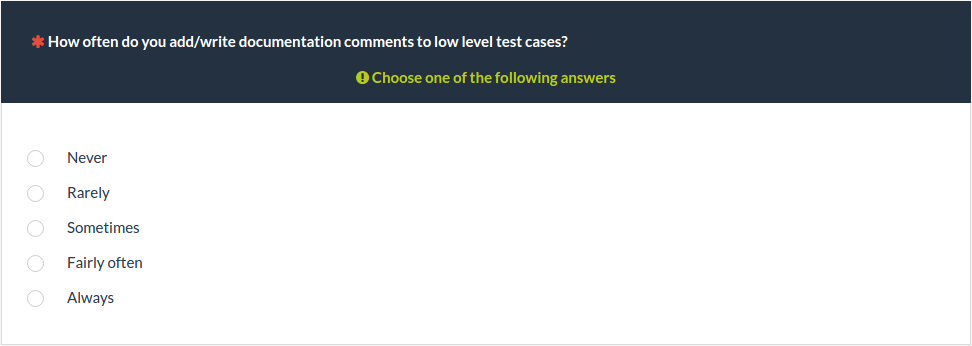
\includegraphics[width=13.7cm]{images/survey-org-comments.png}
        \caption{JUnit survey 5 point scale Likert question}
        \label{fig:survey-junit-comments}
      \end{center}
    \end{figure}
    \begin{addmargin}[0em]{0em}
    \end{addmargin}
    \begin{figure}[ht]
      \begin{center}
        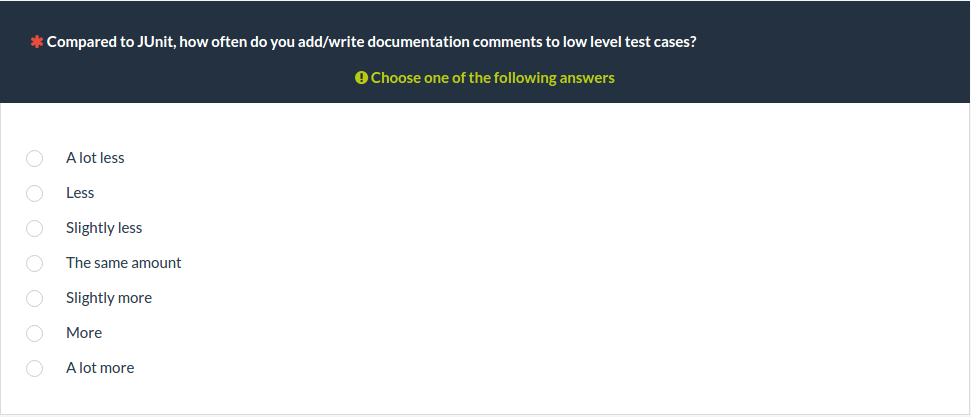
\includegraphics[width=13.7cm]{images/survey-bdd-comments.png}
        \caption{Spectrum survey 7 point scale Likert comparison question}
        \label{fig:survey-bdd-comments}
      \end{center}
    \end{figure}

    The reason to change the questions was to provide direct comparison between the test frameworks.
    If the same question set was repeated to gather insight on the new BDD-testing framework, there exists the risk that
    the participant doesn't remember what he or she answered the last time. It could result in choosing the same answer option,
    despite the slight change in practice or perception in testing.

    The used question types were mostly 1 to 7 point Likert scale questions for the direct comparisons, combined with a few NPS questions for
    determining developer loyalty towards low-level automated testing in general and also towards the new BDD-testing framework.
    A few other type of questions were also added.
    The survey questions and how they are related to research survey questions and related research can be found
    in Appendix \ref{chapter:surveys} section \ref{section:bdd-survey}.

    \subsubsection{Interview about benefits and drawbacks of new BDD-testing framework}
    At the end of the two month data collecting period, a loosely structured semi-structured interview was conducted with the participants
    to get more input on the change period. The interview holds only three basic questions to start with:
    \begin{enumerate}
    \item \textit{What were the main benefits of the new testing framework X over JUnit?}
    \item \textit{What were the main drawbacks of the new testing framework X over JUnit?}
    \item \textit{How long was the learning curve to feel effective with framework X?}
    \end{enumerate}
    The idea to practice these questions with a interview, instead of survey questions, was to lead the discussion
    to possible new topics on the subject if they rose upon interviewing. Also some clarifications were asked to interesting
    answers on the second survey questions. Framework X part of the question relates
    to chosen BDD-testing framework in the project, as it was not the same for both projects.

    \subsubsection{Test code analysis}
    \label{subsub:test}
    Research question 3 is answered with test code analysis done with observation metrics from actual test data of the projects.
    First the baseline is calculated from existing automated low-level tests with JUnit. Second, the same values are calculated
    after the two months period of using an implementation level BDD-testing framework. These metric values are then compared
    against each other, to see how the following aspects of test code have changed:
    \clearpage
    \begin{addmargin}[0em]{0em}
    \vspace{10px}
    \textbf{Automated unit testing level metrics}
    \vspace{5px}
    \newline
    \begin{enumerate}
    \item \textit{Count of test methods \textbf{(COTM)}}:
    Average count of test methods per class method (COTM) is defined at unit level. This is calculated through the sum
    of unit test methods (UTM) divided by sum of class methods under test (CMUT). Data driven test methods add to sum of UTM as
    many separate methods as the the runner produces from it, for instance one data driven test method can produce 20 methods to UTM sum.
    \begin{align*}
        \sum_{i=1}^{n}\frac{UTM_{i}}{CMUT_{i}} && \text {where } UTM_{i} \geq 1 \text{ and } CMUT_{i} = 1
    \end{align*}
    \item \textit{Code coverage \textbf{(CC)}}:
    Measured code coverage for unit tests is done with \textit{JaCoCo}~\cite{jacoco}. The code coverage is measured with
    \textbf{instruction coverage} and \textbf{branch coverage} percentages~\cite{jacoco-coverage}. Instruction coverage counts the percentage
    of hit-and-miss for Java byte code instructions by unit tests. Branch coverage calculates the number of executed or missed \textit{if}
    and \textit{switch} statements by unit tests.
    \end{enumerate}
    \end{addmargin}

    \begin{addmargin}[0em]{0em}
    \vspace{10px}
    \textbf{Automated unit \& integration testing level metrics}
    \vspace{5px}
    \newline
    \begin{enumerate}
    \setcounter{enumi}{2}
    \item \textit{Code coverage \textbf{(CC)}}:
    Measured code coverage for low-level tests is done with \textit{JaCoCo} in the same manner as described earlier in
    unit level code coverage definition. It includes both unit and integration level test coverage.

    \item \textit{Count of Assertions \textbf{(COA)}}:
    Average count of assertions per test method (COA) is defined for low-level test methods. This is calculated with
    the sum of assertions (A) in low-level test methods divided by the total sum of low-level test methods (LLTM).
    \begin{align*}
        \sum_{i=1}^{n}\frac{A_{i}}{LLTM_{i}} && \text {where } A_{i} \geq 0 \text{ and } LLTM_{i} = 1
    \end{align*}

    \item \textit{Count of Comments \textbf{(COC)}}:
    Average count of comments per test method (COC) is defined for low-level test methods. This is calculated with the
    sum of comments (C) in low-level test methods divided by the total sum of low-level test methods (LLTM). Comments include both
    \textit{inner} and \textit{outer} comments. Inner comments are inside the test method and outer comments preceding the test method.
    \begin{align*}
        \sum_{i=1}^{n}\frac{C_{i}}{LLTM_{i}} && \text {where } C_{i} \geq 0 \text{ and } LLTM_{i} = 1
    \end{align*}

    \item \textit{Test method name word count \textbf{(TMNWC)}}:
    Average test method name word count (TMNWC) is counted differently for different testing frameworks.

    For \textbf{JUnit} low-level test method name words are gathered through splitting the \textit{CamelCase}~\cite{wiki:camelcase}
    method name into separate words. For instance, example test method definition at line 36 in figure \ref{fig:junit-examples}:


    \begin{addmargin}[0em]{0em}
    \vspace{10px}
    \textit{public void testStartGameWithNormalDifficulty()}
    \newline
    \end{addmargin}
    is parsed into a 6 word test method name:
    \begin{addmargin}[0em]{0em}
    \vspace{10px}
    \textit{test Start Game With Normal Difficulty}
    \newline
    \end{addmargin}

    For \textbf{xSpec family} low-level test method name is counted starting from the first code example group description string,
    concatenating nested example group string descriptions and ending in the code example description string.
    For example figure \ref{fig:rspec-example} first concatenated code example name (with word count of 11) is:

    \begin{center}
    \textit{Java::FiAaltoEkanbanServices::GameService startGame() with normal difficulty should create game with given name}
    \end{center}

    For \textbf{\textit{Spock}} low-level test method name is counted from feature method string name. For example DDT feature method name at
    line 27 in figure \ref{fig:spock-example}:
    \begin{center}
    \textit{GameService startGame() with playerName \#playerName and difficulty \#gameDifficulty}
    \end{center}
    contains 8 words.

    For each testing frameworks, TMNWC is calculated through the sum of test method name words (TMNW) divided by total sum of low-level test methods (LLTM).
    \begin{align*}
        \sum_{i=1}^{n}\frac{TMNW_{i}}{LLTM_{i}} && \text {where } TMNW_{i} \geq 1 \text{ and } LLTM_{i} = 1
    \end{align*}

    \item \textit{Data driven test methods \textbf{(DDTM)}}:
    DDTM, Ratio of data driven low-level test methods (DDLLTM) to low-level test methods (LLTM) is calculated by dividing the sum
    of DDLLTM by LLTM.
    \[\frac{\sum_{i=0}^{n}DDLLTM_{i}}{\sum_{j=1}^{m}LLTM_{j}}\]
    \end{enumerate}
    \end{addmargin}

\section{Validity and reliability}
In this section, the different categories of validity together with reliability are analyzed with mitigated risks and remaining
threats.
Validity is categorized by aspects recommended by Runeson et al.~\cite{runeson2012case}. Relevant threat categories in
this research include \textit{construct, internal \& external validity} and \textit{reliability} of the study.
First, construct validity is analyzed. Second, internal validity is examined. Third, external validity is studied and
finally reliability is discussed.

\subsection{Construct validity}
The construct validity reflects how well the studied aspects represent the original intention of the researcher~\cite{runeson2012case}.
Threats to construct validity include the threats to validity of the used study methods. Mitigations used for this risk
in study were:
\begin{itemize}
\item Data collection used \textbf{methodological triangulation} with surveys, interviews and test code analysis. Quantative and qualitative data was used.
\item Large parts of survey regarding the developer practices and perception towards \textit{JUnit} were well-founded
by using previous research survey questions as the starting base directly.

\item Code analysis metrics such as \textit{COTM} or \textit{COA} were defined clearly.

\item Risk in understanding of surveys was mitigated by providing support available for the participants during the answering
of the survey to avoid misunderstood questions.

\end{itemize}

\noindent However, there is still a probability
that the survey question was not interpreted the same way as it was intended to study the aspects of testing. Interview questions
were understood seemingly correct, as the interview situations and discussions gave better insight to developer answers.
\subsection{Internal validity}
Internal validity examines the causal relations of the study~\cite{runeson2012case}, the presence of \textit{bias} in the study}~\cite{kitchenham2002preliminary}.
To mitigate respondent bias, \textbf{prolonged involvement}~\cite{runeson2012case} was used in studying participants of the study. During the conducting of the study, I
was employed in the studied company. This enabled the access to project source code for test code analysis and also providing
a trustful relationship with the study participants.

Internal validity threat includes the unexpected sources of bias~\cite{kitchenham2002preliminary}. The before mentioned
prolonged involvement could lead to \textbf{researcher bias}.
Another source of unwanted bias comes from the process of finding relevant projects and teams for the study.
I first had the task of convincing participants to take a new BDD-testing framework into use in the middle of the
project. This process is explained in detail in chapter \ref{chapter:projects}, but it can be summerized as an enthusiastic selling of the
BDD-testing frameworks and their features. This can cause some unwanted \textbf{response bias} influenced by a presence
of a \textbf{"champion"}~\cite{kitchenham2002preliminary} driving the change and initial impressions.

\subsection{External validity}
External validity reflects how well the findings in the study can be generalized and how they could interest other people
outside the study~\cite{runeson2012case}. To mitigate the risks to external validity, there was kept attention in
studying the BDD-testing tools in relevant industrial context in actual project settings. Study participants were also selected from senior
developers with same degree experience level. \textbf{Data triangulation} was also used to study the applicability of BDD
tools in different projects with multiple participant data sources.

External validity threats are related to threats that hinder the possibility to generalize the findings from this study~\cite{runeson2012case}.
The demographics which the study was applied can be found in section \ref{section:demographics}. Major threat to generalizing the findings
is the \textbf{limited number of participants} involved through the projects A and B. Projects are demonstrated in detail in section \ref{section:demographics},
but in brief, the participant number in total in them was only 3. As the sample size is small, the results can't be generalized
with certainty to all industrial developers. For example the survey regarding practices and perception towards \textit{JUnit} can
only offer insight to participant working practices, but can't be used to state a generalizations of unit and integration
testing practices amongst majority of developers.
The survey regarding changes in low-level testing after introduction of the implementation level BDD framework in project acts
as a valuable developer experience report with its direct comparison questions, but isn't statistically relevant.

Another problem in generalization is the fact that the study was conducted within Java-projects and JVM-environment, thus this
study is \textbf{specific} to the studied \textbf{environment} and generalizations to other environments can't be made directly.
Additional threats to external validity were the short
\textbf{limited} two months period of \textbf{time} were the study was conducted and the \textbf{limited amount of new test cases} studied
in the test code analysis part of the research.

\subsection{Reliability}
Reliability of this study is the aspect of the study being dependent on the researcher~\cite{runeson2012case}. The study
research methods and especially data collection methods are explained in detail and thus they should be able to be replicated by other researchers.
Also the source code for enabling needed build configurations and test framework extensions are provided.

One aspect that hinders the reliability is the provided refactoring of \textit{JUnit} tests to BDD-testing framework examples explained
in chapter \ref{chapter:projects}. This step is hard to reproduce by other research on a larger scale, as it involves time and effort not
possibly available. This example providing can also cause bias in the studying by
shifting the written new tests to a certain structure that supports the research hypothesis. Although providing examples
of good practices should only help to produce test code closer to as originally intended by the authors of these BDD-testing framework creators.

This chapter discussed the case study details; what was studied and how it was done. Before chapter \ref{chapter:results} and case study results,
the next chapter illustrates how selected project teams chose their new implementation level BDD-testing framework to take in use.



